\section{CMB transfer observables and initial-state dependence}\label{sec:cmb}

\subsection{Acoustic scale and thermal history}\label{sec:acoustic-scale}
For the Planck-normalized spatially flat reference model, photon-baryon sound speed and sound horizon obey
\begin{align}
c_s(a)&=\frac{c}{\sqrt{3[1+R_b(a)]}},\qquad R_b(a)=\frac{3\Om_b}{4\Om_\gamma}a,\\
r_s(z_*)&=\int_0^{a_*}\frac{c_s(a)}{a^2H(a)}\dd a,\\
D_M(z_*)&=c\int_0^{z_*}\frac{\dd z}{H(z)},\quad \theta_*=\frac{r_s(z_*)}{D_M(z_*)},\quad \ell_A=\frac\pi{\theta_*}.
\end{align}
Taking $z_*=1089.92$ as an \emph{external recombination input}, our integrations return
\begin{equation}
\boxed{\begin{aligned}
r_s(z_*)&=144.294\ \Mp,&D_M(z_*)&=13864.38\ \Mp,\\
100\theta_*&=1.04075,&\ell_A&=301.86.
\end{aligned}}
\end{equation}
The inferred Planck acoustic-angle reference is $100\theta_*=1.0411\pm0.0003$ \cite{Planck}. The present value is conditional on the supplied $z_*$, densities and $H_0$, and tests this approximate background geometry. The quantity $\ell_A$ is the acoustic spacing; radiation driving and phase shifts place the first TT peak near $\ell\sim220$.

\subsection{Temperature, polarization, and lensing spectra}\label{sec:cmb-state}
Temperature and polarization observables combine their transfer functions with a specified primordial state. A convenient primordial parameterization is
\begin{equation}
\mathcal P_{\mathcal R}(k)=A_s\left(\frac{k}{k_0}\right)^{n_s-1+\frac12\alpha_s\ln(k/k_0)+\cdots}.
\end{equation}
The baryon loading determines odd/even peak heights, gravitational potential evolution and neutrino free streaming control acoustic phases, photon diffusion causes Silk damping, and Thomson scattering generates polarization. A kinetic recombination solution evolves the ionization fractions and matter temperature together. Reionization and optical depth $\tau_{\rm reio}$ then modify large-scale E modes and damp primary small-scale anisotropies. The observational Planck baseline gives $\Om_bh^2\simeq0.02237$, $\Om_ch^2\simeq0.1200$, $n_s\simeq0.965$ and $\tau_{\rm reio}\simeq0.054$ \cite{Planck}.
Hydrogen Saha equilibrium gives an explicit thermodynamic reference:
\begin{equation}
\frac{x_e^2}{1-x_e}=\frac1{n_H}\left(\frac{m_ek_BT}{2\pi\hbar^2}\right)^{3/2}\exp\!\left[-\frac{13.5984\,\mathrm{eV}}{k_BT}\right].
\end{equation}
For $Y_p=0.245$ and $T_0=2.7255$ K, the equilibrium solution has $x_e=1/2$ at $z\simeq1369$ and $x_e(z_*)\simeq0.00376$. These values describe the equilibrium ionization fraction. Delayed recombination, residual electrons and helium populations are governed by the multilevel-atom rate equations. Their electron density determines the Thomson visibility and the kinetic last-scattering distribution.

\begin{figure}[t]\centering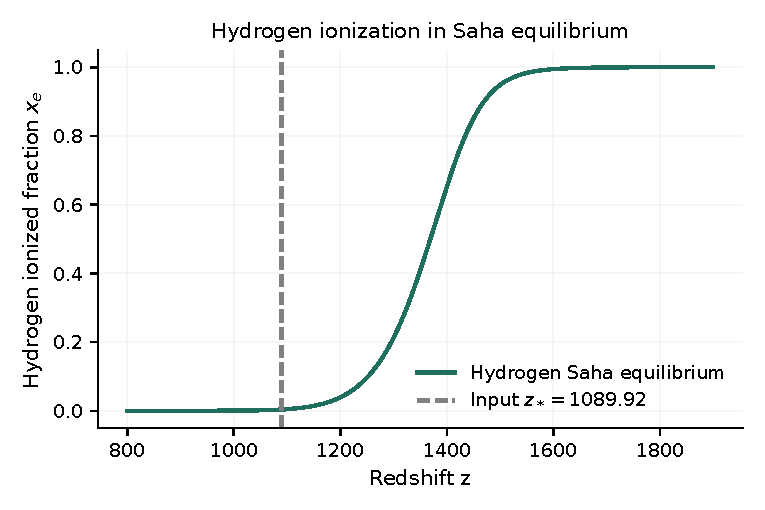
\includegraphics[width=.79\linewidth]{figures/saha_ionization_reference.pdf}\caption{Hydrogen equilibrium ionization history and the independently imposed reference last-scattering redshift. The plotted curve describes Saha equilibrium; visibility is defined by the kinetic electron density.}\end{figure}

The calculated CMB numbers describe acoustic geometry and the equilibrium reference. The temperature, polarization and lensing spectra are analytic functionals of the separately specified primordial measure and kinetic transfer functions.

\subsection{Line-of-sight sources, polarization and diffusion}
\label{sec:cmb-hierarchy}
CMB temperature and polarization power depend on dynamical sources along the photon trajectory. For each Fourier mode, the Einstein--Boltzmann hierarchy evolves the metric and matter fluids, photon temperature and polarization multipoles, baryon velocity, neutrinos, and the recombination visibility function. In the following transfer formulas, conformal time and distance are expressed in units with $c=1$. Under scalar adiabatic initial conditions, the conventional line-of-sight construction may be written \cite{Ma95,Seljak96}
\begin{align}
\Delta_\ell^{T}(k)&=\int_0^{\eta_0}\dd\eta\,S_T(k,\eta)j_\ell[k(\eta_0-\eta)],\\
\Delta_\ell^{E}(k)&=\sqrt{\frac{(\ell+2)!}{(\ell-2)!}}
\int_0^{\eta_0}\dd\eta\,\frac{3g(\eta)\Pi(k,\eta)}{4[k(\eta_0-\eta)]^2}
 j_\ell[k(\eta_0-\eta)],\\
C_\ell^{XY}&=4\pi\int\dd\ln k\,\mathcal P_{\mathcal R}(k)\,\Delta_\ell^{X}(k)\Delta_\ell^{Y}(k),
\qquad X,Y\in\{T,E\},
\label{eq:cl}
\end{align}
The E-mode expression applies for $\ell\geq2$. The transfer $\Delta_\ell^T$ refers to $\Delta T/T_0$ and polarization is in the same temperature normalization, so these $C_\ell$ are dimensionless; multiplication by $(10^6T_0)^2$ gives $\mu\mathrm K^2$. Here $q(\eta)=a n_e\sigma_T>0$, $\tau(\eta)=\int_\eta^{\eta_0}q(\eta^{\prime})\dd\eta^{\prime}$ and $g(\eta)=q(\eta)e^{-\tau(\eta)}$ is the positive Thomson visibility and $\Pi$ is the photon quadrupole polarization source. The expressions include Sachs--Wolfe, integrated Sachs--Wolfe and Doppler terms through $S_T$ once those sources have been calculated. The primordial spectrum $\mathcal P_{\mathcal R}$ specifies the initial-state measure; its provenance is either a stated early-time QICT state or an external cosmological input.

In the tightly coupled epoch the baryon-to-photon inertia ratio $R=3\rho_b/(4\rho_\gamma)$ sets the adiabatic sound speed $c_s^2=1/[3(1+R)]$ in units $c=1$, and the diffusion damping scale is
\begin{equation}
 k_D^{-2}(\eta)=\int_0^\eta\frac{\dd\eta'}{6q(\eta^{\prime})(1+R)}
\left[\frac{R^2}{1+R}+\frac{16}{15}\right].
\label{eq:silk}
\end{equation}
The acoustic separation is approximately $\ell_A=\pi\chi_*/r_s(\eta_*)$; the individual TT peak positions differ from integer multiples of $\ell_A$ because of radiation driving, baryon loading, free-streaming species and projection. Relative peak heights encode the baryon density, matter--radiation equality and primordial tilt. Small-scale damping depends on the ionization history and the polarization collision source. Cosmic lensing remaps the primary sky through the scalar Weyl-potential power along the line of sight. The acoustic geometry and the full TT, TE and EE transfer functions thus represent distinct levels of the calculation.

For completeness, the same scalar metric gives the CMB lensing transfer explicitly. In a spatially flat background and the Born approximation, define $T_{\rm W}$ by $(\Phi+\Psi)(\mathbf k,\eta)=T_{\rm W}(k,\eta)\mathcal R_{\mathbf k}$ in the present $c=1$ convention. With the unobservable angular monopole subtracted inside the line-of-sight integral, the lensing potential and its transfer for $L\geq2$ satisfy \cite{Lewis06}
\begin{align}
\phi(\widehat{\mathbf n})&=-\int_0^{\chi_*}\dd\chi\,
\frac{\chi_*-\chi}{\chi_*\chi}(\Phi+\Psi)_{\rm aniso}(\chi\widehat{\mathbf n},\eta_0-\chi),\\
\Delta_L^\phi(k)&=-\int_0^{\chi_*}\dd\chi\,
\frac{\chi_*-\chi}{\chi_*\chi}T_{\rm W}(k,\eta_0-\chi)j_L(k\chi),\\
C_L^{\phi\phi}&=4\pi\int\dd\ln k\,
\mathcal P_{\mathcal R}(k)|\Delta_L^\phi(k)|^2.\label{eq:cmb-lensing-transfer}
\end{align}
The subscript $\mathrm{aniso}$ denotes subtraction of the angular mean at each distance. The observable deflection is $\nabla_{\widehat{\mathbf n}}\phi$. These relations follow by expanding the line-of-sight Weyl potential in spherical harmonics and applying the primordial covariance. They use the same metric transfer as the temperature and polarization calculation. Their evaluation requires the specified primordial state and transfer evolution.

The transfer integrals define the spectra for a given primordial measure, recombination history and metric response. Their positivity and the information retained by a finite set of angular quantities follow directly.


\subsection{Positivity and the information in finite angular spectra}
\label{sec:cmb-positive}
The transfer representation imposes an exact consistency condition on temperature, polarization and any additional linearly transferred field sharing the same primordial scalar source.
\begin{proposition}[Positive angular covariance]\label{prop:cmb-positive}
For $\mathcal P_{\mathcal R}(k)\geq0$ and square-integrable transfer functions, the matrix
\[
\mathsf C_\ell^{XY}=4\pi\int\dd\ln k\,
\mathcal P_{\mathcal R}(k)\Delta_\ell^X(k)\Delta_\ell^{Y*}(k)
\]
is positive semidefinite. In particular,
\begin{equation}\label{eq:cmb-cauchy}
C_\ell^{TT}\geq0,\qquad C_\ell^{EE}\geq0,\qquad
|C_\ell^{TE}|^2\leq C_\ell^{TT}C_\ell^{EE}.
\end{equation}
For positive diagonal entries, equality holds precisely when the two transfer functions are proportional almost everywhere with respect to the primordial measure.
\end{proposition}
\begin{proof}
For every vector $b$, the quadratic form $b^\dagger\mathsf C_\ell b$ is the integral of $4\pi\mathcal P_{\mathcal R}|\sum_Xb_X^*\Delta_\ell^X|^2$. Positivity and the two-dimensional principal minor give Eq.~\eqref{eq:cmb-cauchy}. Equality is the equality condition in the Cauchy--Schwarz inequality for the two transfer functions. The cross spectrum may have either sign.
\end{proof}

The primordial information retained by a finite set of spectra has an equally precise characterization. For fixed transfer functions, write $m$ measured angular quantities as $c_i=\int K_i(k)\mathcal P(k)\,\dd\ln k$. Suppose an admissible reference spectrum is bounded below by a positive constant on a compact interval. Choose $m+1$ smooth, linearly independent functions $b_j$ supported inside that interval. The $m\times(m+1)$ matrix $A_{ij}=\int K_i b_j\,\dd\ln k$ has a nonzero null vector $v$. Consequently
\begin{equation}\label{eq:primordial-null-family}
\mathcal P_\varepsilon(k)=\mathcal P_0(k)+\varepsilon\sum_{j=1}^{m+1}v_jb_j(k)
\end{equation}
gives the same $c_i$ for all $i$, while sufficiently small $|\varepsilon|$ preserves positivity. Thus finite angular information determines an equivalence class of primordial functions. A finite-dimensional primordial model, such as the power-law parameterization above, selects a specified subfamily for inference. The acoustic geometry, transfer dynamics and primordial measure remain individually defined constituents of each CMB prediction.
